%----------------------------------------------------------
%----------------------------------------------------------
% INTRODUCCIÓN
	"Durante la última década, las universidades pertenecientes al Consejo de Rectores de Universidades chilenas (CRUCH) 
	han promovido diversas iniciativas de Innovación Curricular"\hspace{0.2cm} \cite{INN11}. Es por ello que la Universidad Austral de 
	Chile ya ha empezado con el proceso de innovación curricular para que gradualmente abarque todas sus carreras.
	\\
	
	Uno de los principales problemas relacionados con el proceso de calidad e innovación curricular es que la Universidad 
	Austral de Chile almacena toda la información referente al historial curricular de cada carrera en distintos medios 
	de almacenamiento (incluyendo el papel), distintos  formatos, y en varias unidades de la organización, lo que 
	dificulta la generación de informes que apoyen procesos estratégicos de seguimiento y auto-evaluación.
	\\
	
	Este proyecto surge como una iniciativa de la Dirección de Estudios de Pregrado, donde se observan las dificultades que tienen los 
	departamentos ya indicados previamente, al momento de gestionar documentos relacionados con la innovación curricular.  
	De acuerdo a lo mencionado anteriormente, se pretende crear una plataforma web, que permita gestionar el historial 
	curricular de cada carrera de la universidad, la cual permitirá a distintas Unidades de la universidad tener una 
	mejor información  de las carreras y así facilitar el trabajo que día a día realizan.
	\\
	
	La información obtenida por esta plataforma servirá de apoyo para la gestión curricular por parte de los distintos departamentos que integran la Dirección de Estudios de Pregrado, ya que se contará con todo lo necesario para gestionar los cambios curriculares de los planes de estudio.
	\\


	\subsection{Definición del Proyecto}
	
	\subsubsection{Objetivo general}
	
	Diseñar y construir  un prototipo de una plataforma web que apoye al monitoreo curricular de pregrado. \\
	\vspace{-0.4cm}
	
	\subsubsection{Objetivos específicos}
	
	\begin{itemize}
		\item Conocer cómo los departamentos que integran la Dirección de Estudios de Pregrado (DEP) administran
		la información referente a los planes de estudios.
		\item  Definir requerimientos del sistema, describiendo sus funcionalidades y separar en módulos la aplicación.
		\item Diseñar e implementar el módulo necesario que permita gestionar el historial curricular de una carrera en particular.
		\item Diseñar e implementar el módulo necesario que permita la gestión de documentos.
		\item Realizar pruebas de validación de los requisitos y estabilidad del prototipo de plataforma web.
	\end{itemize}
	
	\subsection{Nivel actual}
	
		Como ya se ha mencionado el presente proyecto pretende aportar a los procesos curriculares de la Universidad Austral de Chile, es por esto mismo que es necesario entender los procesos que realizan los departamentos involucrados.
		\\
		
		En la Figura \ref{Figura1} se puede apreciar como se estructuran los departamentos de Vicerrectoría. A partir de este diagrama se explicarán las principales funciones y procesos de los Departamentos de Estudios de Pregrado, los cuales son: Departamento de Aseguramiento de la Calidad de la Docencia e Innovación Curricular, Departamento de Admisión y Matricula y Departamento de Registro Académico Estudiantil.
	
		\begin{figure}[h]
			\centering
			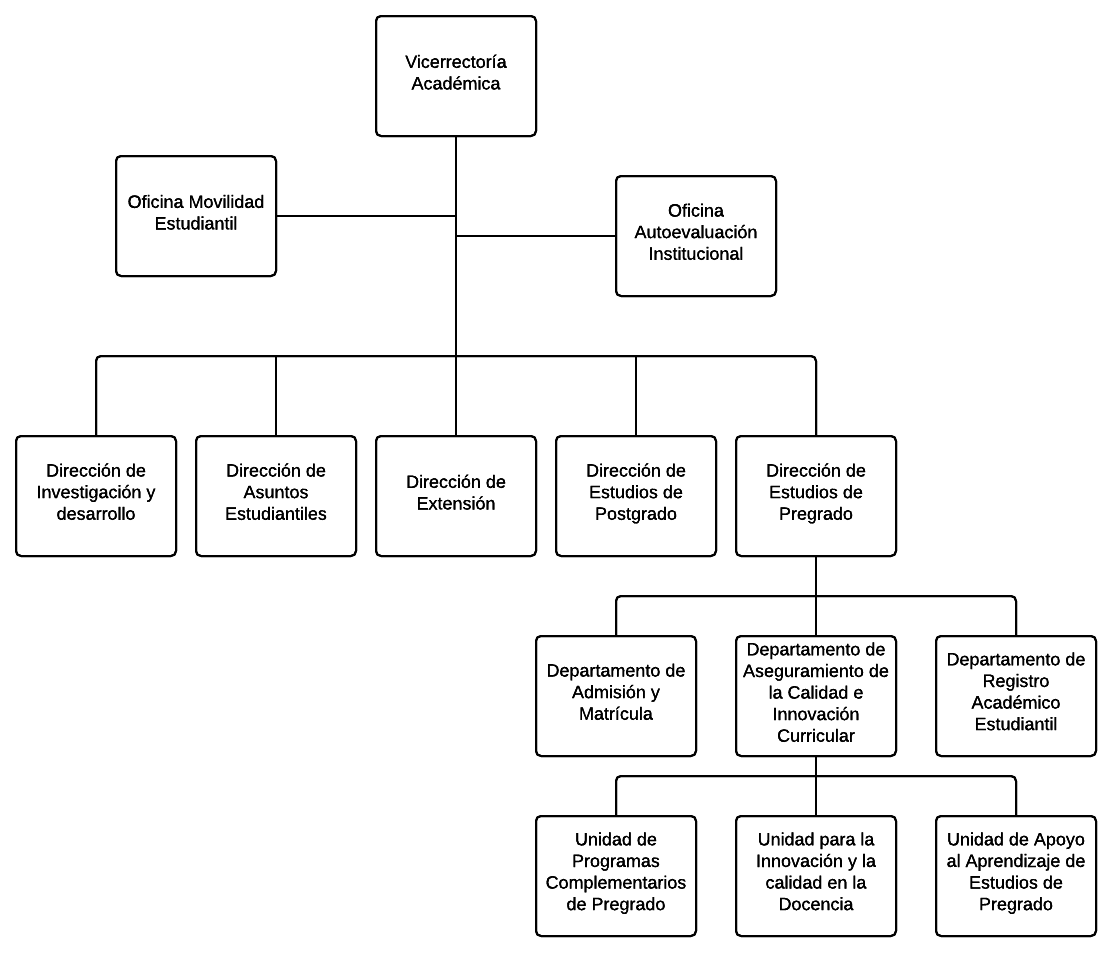
\includegraphics[width=1\textwidth]{images/Capitulo_1/Organigrama.png}
			\caption[Organigrama Vicerrectoría y DACIC]{Organigrama Vicerrectoría y DACIC \footnote{}}
			\label{Figura1}
		\end{figure}
		\footnotetext{Elaboración propia.}
		
		\subsubsection{Departamento de Aseguramiento de la Calidad e Innovación Curricular (DACIC)}
		
		
		En este departamento nace la idea de desarrollar un sistema que apoye a los procesos curriculares. Su principal objetivo es ``propender al fortalecimiento de la calidad de los aprendizajes de los estudiantes de la UACh a través del apoyo a los  Docentes en el diseño de situaciones de enseñanza/aprendizaje orientadas a la obtención de resultados efectivos y el asesoramiento a las unidades académicas respectivas en el desarrollo de innovaciones curriculares."\hspace{0.2cm} \cite{Dac15}
		\\
		
		El departamento está conformado por cuatro Unidades:
			\begin{itemize}
				\item Unidad de Apoyo al Desarrollo de la Docencia de Pregrado
				\item Unidad de Apoyo al Desarrollo y la Innovación Curricular en Pregrado
				\item Unidad de Apoyo al Aprendizaje del Estudiante de Pregrado 	
				\item  Unidad de Programas Complementarios
			\end{itemize}
		
		Sin embargo el proyecto beneficiará directamente  a la Unidad de Apoyo al Desarrollo y la Innovación Curricular en Pregrado, por lo que se dará mas detalles de esta Unidad a continuación.
		
		
		\myparagraph{Apoyo al Desarrollo y la Innovación Curricular en Pregrado}
		
		Unidad encargada de apoyar en el ámbito ``técnico-curricular a las escuelas de Pregrado en sus proyectos de innovación curricular, tanto en carreras profesionales como técnicas, en el contexto del Modelo Educativo y Enfoque Curricular de la Universidad."\hspace{0.2cm} \cite{Dac15}
		\subsubsection{Departamento de Admisión y Matrícula}
		Es la Unidad encargada del proceso de ingreso de los alumnos vía PSU a cada una de las carreras de Pregrado que ofrece la universidad Austral de Chile. Es decir, es la unidad que está presente en la gestión de los procesos de ingresos a la Universidad.\\
		
		Existen dos modalidades para ingresar a la Universidad Austral de Chile, las cuales son:
			\begin{itemize}
				\item Sistema regular, común a toda la Educación Superior adscrita al Consejo de Rectores de las Universidades Chilenas.
				\item Sistema de Ingreso Especial, propio de la Universidad.
			\end{itemize}
			
			\myparagraph{Servicios estudiantiles} 
		
			\begin{itemize}
				\item 	`` El Departamento de Admisión y Matrícula es la Unidad encargada de otorgar las certificaciones de Alumno Regular a todos los estudiantes de la Universidad, que cumplan con los requisitos para la de emisión de dichos documentos."\hspace{0.2cm} \cite{Dep15}
				\item Gestiona  la construcción y entrega de las Credenciales Universitarias.
			\end{itemize}
			
		
		
		
		\subsubsection{Departamento de Registro Académico Estudiantil}
		
		Este departamento depende directamente de la Dirección de Estudios de Pregrado de la Vicerrectoría Académica, está actualmente a cargo de la Srta. María Cristina Barriga Ramírez. Entre sus funciones se destaca ``el seguimiento académico del estudiante de pregrado, postítulo y postgrado desde su primera matrícula hasta su egreso y posterior titulación y/o graduación y el permanente apoyo a la labor administrativa que realizan Directores de Escuela, Directores de Unidades Académicas y Profesores en general"\hspace{0.2cm} \cite{Dir15}.
		
		
		
		
		
		
		\myparagraph{Procesos}
		
		Esta Unidad  controla la información académica - administrativa, prepara y supervisa los siguientes procesos:
		\begin{itemize}
			\item Peticiones de asignaturas que realizan las Escuelas.
			\item Oferta de asignaturas de las Unidades Académicas.
			\item Inscripción de asignaturas de los estudiantes.
			\item Ingreso de las calificaciones por parte de los profesores.
			\item Modificaciones curriculares de los planes de estudios, de acuerdo  a lo aprobado por la Dirección de Estudios de Pregrado.
			
		\end{itemize}
		
		
		Una vez nombrado los diferentes procesos que controla este departamento, se procederá a explicar los dos  principales procesos que están directamente relacionado con el sistema, los cuales son: Creación de nuevas Carreras y  Modificaciones curriculares de los planes de estudios, de acuerdo  a lo aprobado por la Dirección de Estudios de Pregrado.
		
		\myparagraph{Creación de nuevas Carreras}
		
		En el diagrama de procesos que se muestra en la Figura \ref{FiguraDOSCSM} describe la secuencia básica que se lleva a cabo para la creación de nuevas carreras en la Universidad Austral de Chile.
\\
		
		Las fechas para la presentación de nuevos proyectos o innovaciones curriculares, se estipulan en el Decreto de Rectoría  que promulga el Calendario Académico cada año. Para el año 2015 se especifica:
			\begin{itemize}
			\item 30 de abril, último día para presentar en la Vicerrectoría Académica, los proyectos de nuevas carreras.
			\item 30 de junio, último día para que las facultades y sedes presenten proyectos de Innovación Curricular de las carreras a la Vicerrectoría Académica.
		\end{itemize}
		
			\begin{figure}[H]
			\centering
			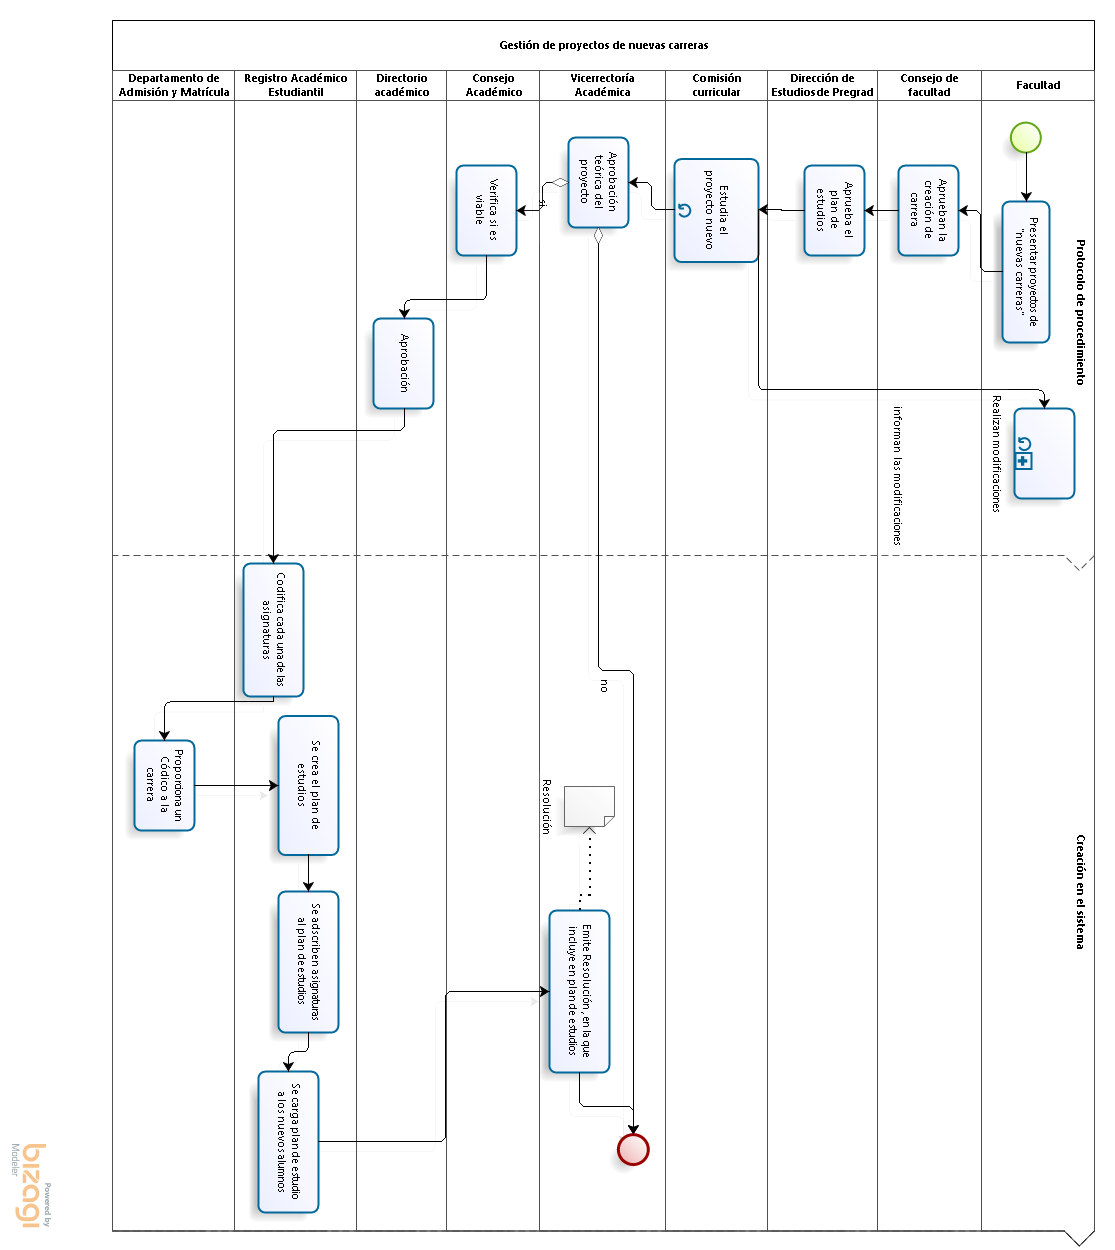
\includegraphics[width=1\textwidth]{images/Capitulo_1/Procesos_Registro_academico.png}
			\caption[Proceso de presentación de nuevos proyectos]{Proceso de presentación de nuevos proyectos \footnote{}}
			\label{FiguraDOSCSM}
		\end{figure}
		\footnotetext{Elaboración propia.}	
			

		
		Una vez aprobado una nueva carrera o la innovación curricular por parte de la Vicerrectoría Académica, los pasos administrativos, son los que se indican a continuación:
		
		
		
		
		\begin{enumerate}
			
			
			\item Se codifica cada una de las asignaturas, asociándose a una Unidad Académica especifica. La Unidad Académica es la que le asigna la sigla, en letras y la numeración es un correlativo que se utiliza para la identificación de la asignatura. Ejemplo: CAEV222-14.
			\\
			CAEV = Ciencias Ambientales y evolutivas (Unidad Académica)
			\\
			222   = Numeración asignada para identificarla dentro de la misma unidad.
			\\
			-14    = año de creación (2014)
			
			\item El Departamento de Admisión y Matrícula proporciona  un código a la carrera. Ejemplo 1826, Escuela de Psicología (valdivia).
			
			\item Una vez que las carreras estén creadas y las asignaturas asociadas a una unidad académica, el Departamento de Registro Académico Estudiantil crea el plan de estudios (ver Figura \ref{Figura2}) con la descripción del propio plan:Nombre de bachillerato,Duración, Año de creación,e etc.
			
			\item El proceso final para la creación de una carrera, es cargar  las asignaturas al plan previamente creado, los pasos son los siguientes:
			\begin{enumerate}
				\item Se ingresa una a una las asignaturas previamente creadas.
				\item Se asocia a un semestre en particular.
			\end{enumerate}
		\end{enumerate}

		\myparagraph{Modificaciones Curriculares Mayores y/o Menores}
		
		Tanto la creación de nuevas carreras como todo lo que tiene que ver con modificaciones con respecto al plan de estudios, son proceso que ve el DACIC, específicamente el sub-departamento de Unidad de Apoyo al Desarrollo y la Innovación Curricular en Pregrado, en conjunto con Registro Académico Estudiantil.
		\\
		
		La Figura \ref{Figura2} muestra los procesos administrativos que realiza Registro Académico Estudiantil, a continuación se explicará con mayor detalle.
		El proceso de modificación del plan de estudios comienza con la iniciativa de una escuela, la cual se reúne previamente con Registro Académico Estudiantil, con el objetivo  de identificar quiénes son los afectados por los cambios (número de alumnos, año de ingreso, plan de estudios, etc.). Una vez concretada esta reunión, la escuela se encuentra en condiciones de formalizar la petición, la cual es enviada a Dirección de Estudios Pregrado con la intención de que sea evaluada. En caso de que la petición sea viable, Dirección de Estudios de Pregrado envía una comunicación interna a Registra Académico Estudiantil, informándole que puede efectuar los cambios.
		\\
		
				Por último Registro Académico Estudiantil realiza una petición de requerimientos a la DTI (en caso de que sea necesario, de lo contrario no se efectúa este proceso) para posteriormente aplicar los cambios e informarle a la escuela si Dirección de Estudios Pregrado rechazó o aprobó las modificaciones curriculares.
		\begin{figure}[H]
			\centering
			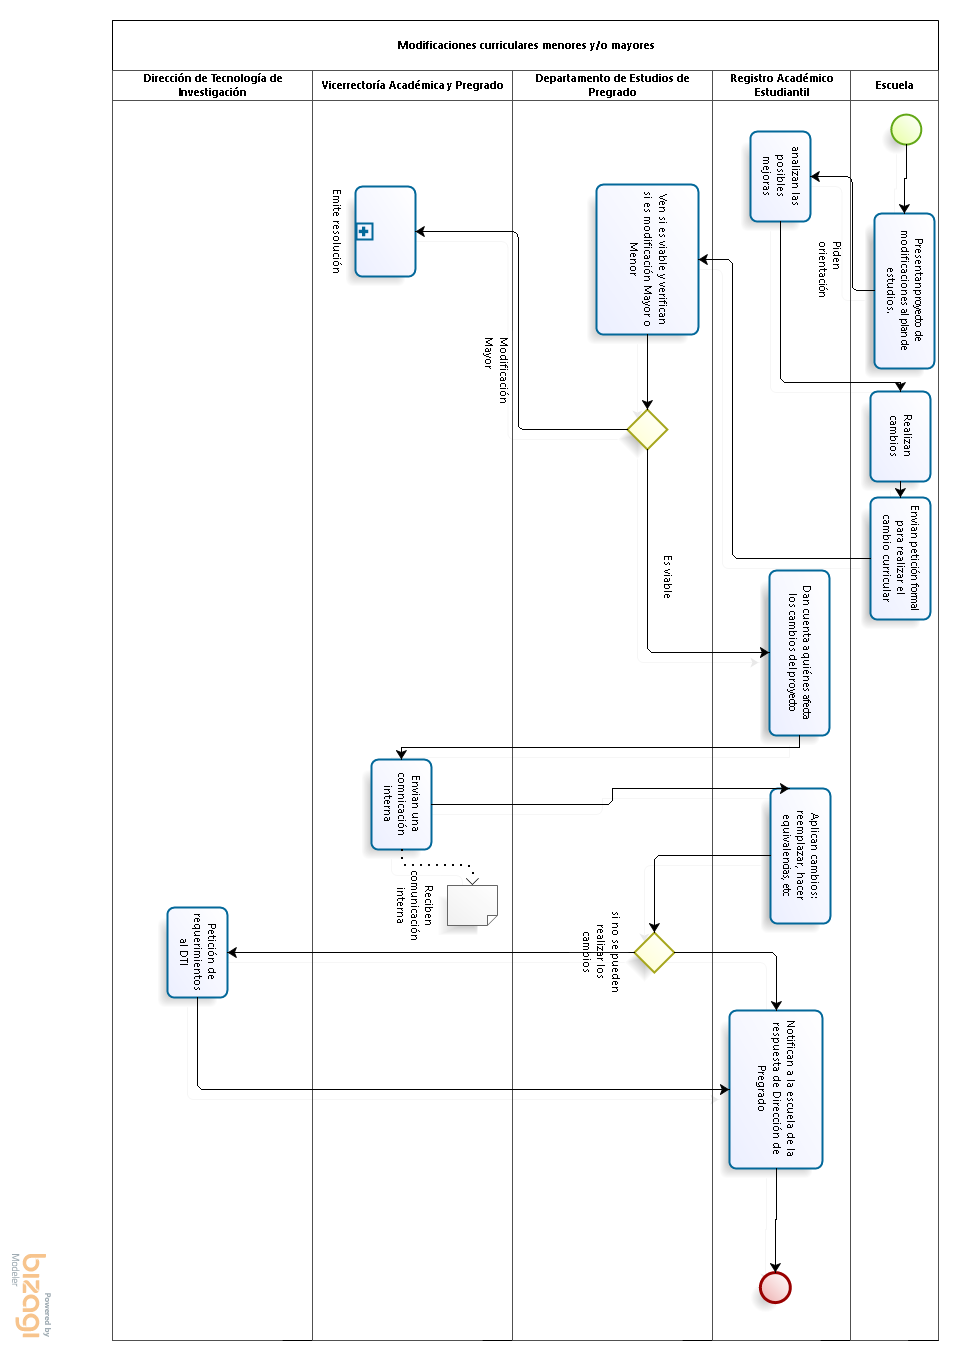
\includegraphics[width=1\textwidth]{images/Capitulo_1/Procesos_cambios_curriculares.png}
			\caption[Procesos de cambios Curriculares Mayores y/o menores ]{Procesos de cambios Curriculares Mayores y/o menores  \footnote{}}
			\label{Figura2}
		\end{figure}
		
		\footnotetext{Elaboración propia.}		
		

		
		
		\newpage
		
		
		Dado lo anterior, podemos ver que los procesos curriculares no se gestionan con un sistema informático, no existiendo un software encargado  de almacenar y documentar los cambios que afectan a los proyectos curriculares de las carreras.
		
	
\subsection{Metodología}

Para cumplir con los objetivos de este proyecto, es necesario adquirir conocimientos de los procesos administrativos de los departamentos involucrados en el proyecto, lo cual permitirá entender cómo estas oficinas manipulan la información referente a los planes de estudio.
\\

Para conocer los procesos mencionados anteriormente, se debe trabajar en conjunto con el DACIC, el cual proporcionará toda la información bibliográfica relacionada con los cambios de las mallas curriculares, es decir; resoluciones, diagrama de procesos, formularios de programas innovados, etc.
\\

Para finalizar la etapa teórica, se investigó sobre las tecnologías en las cual se desarrollará el software, que como ya se ha mencionado anteriormente, las tecnologías asociadas al proyecto tienen que ser compatibles con las que usa la Universidad Austral de Chile.
\\


La siguiente etapa del proyecto, es diseñar y desarrollar el software. Para esta etapa se definió una metodología de entrega incremental, ya que en un principio los requisitos no estaban muy claros al comienzo del proyecto. El desarrollo se dividió en tres incrementos. En el primer incremento se seleccionaron los requisitos que se relacionaban con la gestión del historial curricular de una carrera en particular,  el segundo incremento se seleccionan los requisitos referentes a la gestión de documentos, por último, el tercer incremento  corresponde a la Autentificación y gestión de perfiles de usuarios.
\\

Para finalizar, se realizó una etapa de validación del software, donde se probó la funcionalidad y usabilidad de éste, con el fin de comprobar si cumplía con los requisitos propuestos. Para validar las funcionalidades esperadas del software y la usabilidad del mismo, se trabajo con la Sra. Pilar Alarcón, secretaria de Registro Académico Estudiantil, quien utilizó el software y ayudó a poblar el sistema desarrollado.

